\documentclass[5p,12pt]{elsarticle}

\usepackage{amssymb}
\usepackage{amsthm}

\journal{Nuclear Physics B}

\begin{document}

\begin{frontmatter}

\title{Spectroscopic information about a hypothetical tetrahedral configuration in $^{156}Gd$}

\author[ipnl]{Q. T. Doan\corref{cor1}}
\ead{qtdoan@gmail.com}
\author[ipnl,ucbl]{O. Stezowski}
\author[ipnl,ucbl]{D. Guinet}
\author[iphc]{J. Dudek}
\author[iphc]{D. Curien}
\author[pan]{N. Schunck\fnref{fn1}}

\address[ipnl]{Institut de Physique Nucl\'eaire de Lyon, France}

\address[ucbl]{Universit\'e de Lyon, Universit\'e Lyon 1, Lyon, France}

\address[iphc]{Departement de Recherches Subatomiques, Institut Pluridisciplinaire Hubert Curien, Strasbourg, France}

\address[pan]{Institute of Nuclear Physics PAN, PL-31-342 Krak\'ow, Poland}

\cortext[cor1]{Corresponding author}
 
\fntext[fn1]{Present address: Lawrence Livermore National Laboratory, L-414, P.O. Box 808, Livermore, CA 94551, USA}

\begin{abstract}
A detailed $\gamma$-ray spectroscopy of the lowest two negative-parity bands in $^{156}$Gd has been performed ...
\end{abstract}

\begin{keyword}
$\gamma$-ray spectroscopy \sep $^{156}$Gd
\end{keyword}

\end{frontmatter}



\section{Introduction}
\label{sec:intro}

Theoretical studies based on the nuclear mean-field approach and group theory considerations suggest \cite{bib_dudek2006, bib_schunk2006} that some atomic nuclei may exhibit tetrahedral and/or octahedral symmetries. To the lowest order, tetrahedral symmetry is realized through octupole deformation $Y3\pm 2$ of the nuclear surface. Previous research\cite{bib_dudek2002} has determined magic numbers for which tetrahedral deformation should be the easiest to observe leading to tetrahedral proton and neutron "magic" numbers Zt/Nt = 32, 40, 56, 64, 70, 90, and 112, with extra gaps at Nt = 136 and 142. The authors of Refs. \cite{bib_dudek2006, bib_schunk2006, bib_dudek2002} have furthermore demonstrated that nuclei with an exact tetrahedral symmetry have all multipole moments $Q_\lambda < 7$, $\nu = 0$ except for $Q_{32}$ - thus, in particular, the corresponding quadrupole moments $Q_2$ vanish.
...............
The radiation intensity can be written down using the standard expression in the Equation \ref{equa:distr}.

\begin{equation}
\label{equa:distr}
I(\theta) = 1 + A_{2}P_{2}(\cos{\theta}) + A_{4}P_{4}(\cos{\theta})
\end{equation}

...............

\section{Experiment setup}

\begin{figure}[!htb]
\centering
	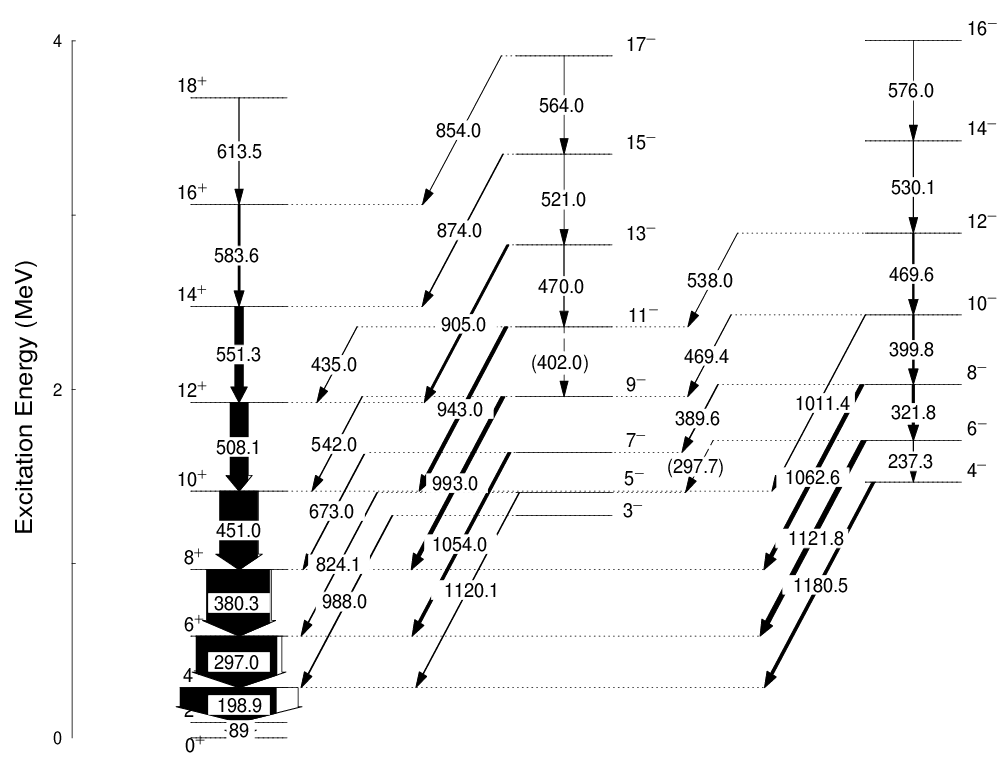
\includegraphics[width=0.5\linewidth]{156Gd.png}
	\caption{Partial level scheme of 156Gd.}
	\label{fig:156Gd}
\end{figure}

...............

\section{Spectroscopy information}
Transition intensities are presented in the Figure \ref{fig:156Gd} ... 

\section{Acknowledgements}

Thiswork benefited from the TNT2-D cards, developed and financed by CNRS/IN2P3 for the GABRIELA project ...


\appendix
\section{Experiment data}
\label{app:expdata}

Experiment data are shown in the Table \ref{tab:data} ... 

\begin{table}[!htb]
\centering
	\caption{Data $\gamma$ ray detection.}
	\label{tab:data} 
	\begin{tabular}{ccc}
		\hline
		Interaction	& Clover 	& Cluster\\
		\hline
		1	& 74.5 & 79.8\\
		2	& 22.4 & 18.3\\
		$\ge$3	& <3.3 & <2.8\\
		\hline
	\end{tabular}
\end{table}


\section*{References}
\bibliographystyle{elsarticle-num} 
\bibliography{biblio}

\end{document}
\endinput